\shorthandoff{"}
\chapter{Methodik}
\label{ch:methodik}

\section{Art der Forschung}
\label{ch:methodik:art}
Um die Forschungsfrage dieser Master-Thesis zu beantworten, wird eine quantitative Forschungsarbeit in Form eines Experiments durchgeführt. In diesem Kontext werden zwei Versionen eines Empfehlungssystems zur Besetzung offener Projektpositionen entwickelt. Eine der beiden Anwendungen verfolgt einen unilateralen, die andere einen bilateralen Ansatz. Beide Empfehlungssysteme erhalten dieselben offenen Projektpositionen und Mitarbeiter als Eingabe. Anschließend sortieren sie die vorhandenen Angestellten für die offenen Stellen und geben diese in Form von Listen zurück.

Die Ausgaben beider Systeme werden Projektmanagern vorgelegt. Diese bewerten für jede Liste auf einer vordefinierten Skala, welche Arbeitsleistung sie von denen in der vorliegenden Reihenfolge dargestellten Mitarbeitern erwarten. Dabei wird evaluiert, ob sie die erwartete Leistung der vorgeschlagenen Angestellten des bilateralen Empfehlungssystems höher bewerten, als die der unilateralen Variante.

Die Mitarbeiter des Unternehmens erhalten Übersichten über offenen Projektpositionen. Daraufhin bewerten sie auf einer vordefinierten Skala, wie zufrieden sie mit einer Tätigkeit auf den vorliegenden Projektpositionen wären. Dabei wird überprüft, ob das bilaterale Empfehlungssystem die Angestellten für die offene Projektpositionen höher positioniert, bei welchen diese eine hohe Zufriedenheit erwarten.
%Abschließend werden die Bewertungen von Projektmanagern und Angestellten hinsichtlich der Ergebnisse der beiden Empfehlungssysteme verglichen. Dabei wird bestimmt, ob die bilaterale Recommender Engine im direkten Vergleich mit dem unilateralen Ansatz sowohl auf Seiten der Projektmanager für eine höhere erwartete Leistung als auch aus Perspektive der Mitarbeiter für eine gesteigerte prognostizierte Zufriedenheit sorgt.

Im Rahmen der vorliegenden Master-Thesis wird ausschließlich der komplementäre \ac{PEFit} auf Facetten-Ebene betrachtet. Hierbei werden einzig die für offene Projektpositionen benötigten Kompetenzen zur Bestimmung der Kongruenz herangezogen. Weitere Faktoren wie Kundennamen, Branche oder Projektbeschreibungen werden nicht berücksichtigt. Im Sinne des ergänzenden \acp{PEFit} wird vorausgesetzt, dass eine Übereinstimmung der Werte von Angestellten und des Unternehmens bzw. der Projekttätigkeiten bereits vor Anstellung der Arbeitnehmer überprüft wurde. Aus diesem Grund wird dieser im Experiment nicht untersucht.

\section{Versuchsaufbau}
\label{ch:methodik:versuchsaufbau}
Durchgeführt wird das Experiment mit Projektmanagern und Mitarbeitern der EXXETA AG mit Hauptsitz in Karlsruhe. Das Unternehmen ist spezialisiert auf IT-Beratungsleistungen und arbeitet vorrangig projektbasiert. Passende Angestellte zu offenen Projektpositionen zuzuordnen ist in diesem Betrieb dementsprechend eine häufig auftretende Aufgabe.

Die Mitarbeiter der EXXETA AG pflegen ihre Kompetenzen in einem Intranet. Dort steht eine Liste mit 551 Fähigkeiten wie beispielsweise "Java", "DSGVO" und "Digitale Transformation" zur Verfügung. Diese können die Angestellten über die in Abbildung \ref{fig:methodik:versuchsaufbau:daten:abb1} dargestellte Skala bewerten.

\begin{figure}[h]
	\centering
	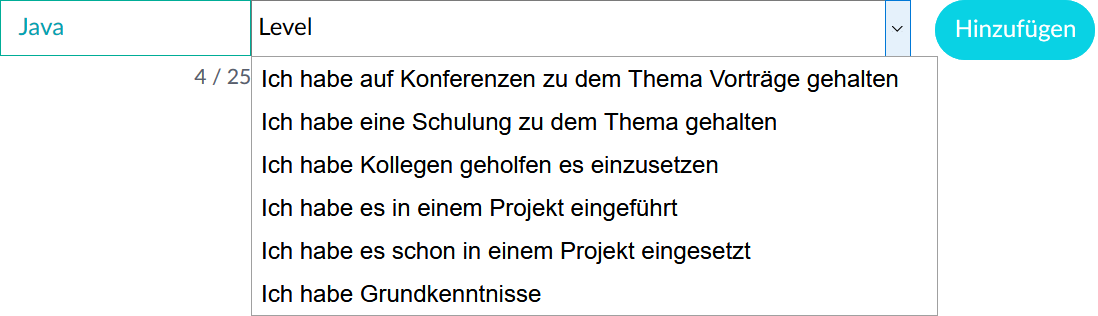
\includegraphics[width=1\textwidth]{gfx/skill-level.png}
	\caption{Hinzufügen einer Fähigkeit mit Angabe des entsprechenden Kenntnisniveaus im EXXETA-Intranet}
	\label{fig:methodik:versuchsaufbau:daten:abb1}
\end{figure}

Die Abstufungen in Abbildung \ref{fig:methodik:versuchsaufbau:daten:abb1} werden beim Speichern in ganzzahlige Werte von 0 ("Ich habe Grundkenntnisse") bis sechs ("Ich habe auf Konferenzen zu dem Thema Vorträge gehalten") übertragen.

Aufgrund der klaren Beschreibungen der einzelnen Stufen in Abbildung \ref{fig:methodik:versuchsaufbau:daten:abb1} kann der in Kapitel \ref{ch:empfehlungssysteme:cf:speicherbasiert} angesprochene Bias bei der Selbsteinschätzung weitgehend ausgeschlossen werden. Außerdem ist es in der vorliegenden Problemstellung gut möglich, dass einzelne Mitarbeiter ihre Kompetenzen bewusst besser oder schlechter einschätzen als andere Kollegen. Dieser Sachverhalt kann insbesondere auf längere Berufserfahrung zurückgeführt werden. Aus diesen Gründen wird bei der Empfehlungsbestimmung auf eine Mittelwert-Zentrierung verzichtet.

Damit Projektmanager Empfehlungen erhalten können, müssen sie die für offene Projektpositionen relevanten Fähigkeiten mitsamt der benötigten Kenntnisniveaus festlegen. Die Kompetenzen bestimmen die Verantwortlichen in der Regel anhand eingehender Projektanfragen, welche Kunden in unstrukturierter Form einreichen. Derartige Anfragen werden täglich in großer Anzahl bearbeitet. Daher wird es für den praktischen Einsatz als sehr umständlich bewertet, wenn Verantwortliche für jede angefragte Projektposition sämtliche Fähigkeiten auf der Skala von eins bis sechs bewerten müssen. Aus diesem Grund werden die Kompetenzniveaus aus Abbildung \ref{fig:methodik:versuchsaufbau:daten:abb1} auf die Abstufungen "Grundkenntnisse" und "Fortgeschritten" vereinfacht. "Grundkenntnisse" entspricht dabei den ersten drei Stufen und "Fortgeschritten" den oberen drei Fähigkeitsniveaus in Abbildung \ref{fig:methodik:versuchsaufbau:daten:abb1}.

Die Kompetenzbewertungen der Mitarbeiter und die für ein Projekt benötigten Fähigkeiten dienen im Experiment als Eingabe für einen grundlegenden Algorithmus, welcher sowohl für das unilaterale, als auch das bilaterale Empfehlungssystem gleich ist.

\subsection{Grundlegender Algorithmus}
\label{ch:methodik:versuchsaufbau:grundlegend}
% Zusätzlich wird das zu besetzende Projekt als Pseudo-Mitarbeiter eingefügt.
Die Mitarbeiter der EXXETA AG und deren Fähigkeiten werden in Form eines Graphen dargestellt. Um das Sparsity Problem zu lösen, wird der speicherbasierte Algorithmus von Katz aus Kapitel \ref{ch:empfehlungssysteme:cf:speicherbasiert} angewendet. Da die Anwendung auch über die Master-Thesis hinaus im Unternehmen eingesetzt werden soll, ist insbesondere die Langlebigkeit des Verfahrens vorteilhaft gegenüber modellbasierten Methoden. Sollten sich nach Durchführung des Experiments Daten im Unternehmen signifikant verändern oder neue Kompetenzen im Intranet hinzugefügt werden, ist der speicherbasierte Algorithmus weiterhin ohne zusätzlichen manuellen Aufwand im Betrieb anwendbar. Die hohe Komplexität ist in der vorliegenden Problemstellung tolerierbar, da sich zum Zeitpunkt des Experiments weniger als 1.000 Mitarbeiter im Unternehmen befinden.

Wie in Kapitel \ref{ch:empfehlungssysteme:cf:speicherbasiert} beschrieben, sorgt der Algorithmus von Katz für eine feingranulare Anpassung vorhandener Beurteilungen. Dass Bewertungen von Mitarbeitern gänzlich fehlen, kann bei er EXXETA AG weitgehend ausgeschlossen werden. Führungskräfte fordern ihre Angestellten regelmäßig dazu auf, ihre Kompetenzen im Intranet aktuell zu halten und diese beispielsweise im Rahmen des Mitarbeiter-Jahresgespräches zu pflegen. Angestellte ohne Bewertungen sind folglich nur in Ausnahmefällen zu erwarten. Hierzu zählen beispielsweise Werkstudenten und neue Mitarbeiter.

Um Kaltstarts auch in solchen Ausnahmefällen vorzubeugen, werden zusätzlich zu den Fähigkeiten der Mitarbeiter auch deren Teamzuordnungen in Form eines hybriden Ansatzes beachtet. Dieses Vorgehen hat außerdem den Vorteil, dass die Kompetenzen der Mitarbeiter bei Berechnung des Algorithmus feingranular besser bewertet werden, wenn ihre direkten Kollegen diese Fähigkeiten ebenfalls beherrschen. Dieses Vorgehen ist im Falle der EXXETA AG als sinnvoll zu bewerten, da dort stets Mitarbeiter mit ähnlichem fachlichem Hintergrund in einem Team tätig sind. Auch der Manager des Teams ist eine fachliche Führungskraft, dessen Fähigkeiten weitgehend repräsentativ für seine Mitarbeiter sind. Seine Kompetenzen sind jedoch in der Regel stärker ausgeprägt.

Die Bewertungen der Fähigkeiten und die Teamzuordnungen können für alle Mitarbeiter der EXXETA AG über eine REST-Schnittstelle in Form von JSON aus dem Intranet abgefragt werden. Einzelne Mitarbeiter sind dabei eindeutig über ihre E-Mail-Adresse identifizierbar. Wäre John Doe aus Tabelle \ref{tbl:empfehlungssysteme:arbeitsweise:tbl1} ein Mitarbeiter des Unternehmens, würden seine zurückgegebenen Daten dem JSON in Listing \ref{qc:methodik:versuchsaufbau:daten:qc1} entsprechen. Nicht relevante Informationen wurden im vorliegenden Auszug entfernt. In diesem und den folgenden Beispielen werden Jane Doe und Max Muster sowie Erika Muster und John Doe als Mitglieder jeweils eines Teams betrachtet. 

%\begin{minipage}{\linewidth}
\lstinputlisting[
language=json,
caption=Beispiel für ein Mitarbeiter-JSON der REST-Schnittstelle des Intranets der EXXETA AG (Auszug),
captionpos=b,
label=qc:methodik:versuchsaufbau:daten:qc1
]{gfx/john.json}
%\end{minipage}

Wie bereits im Kontext von Abbildung \ref{fig:methodik:versuchsaufbau:daten:abb1} erläutert, sind die Bewertungen der Kompetenzen im JSON aus Listing \ref{qc:methodik:versuchsaufbau:daten:qc1} um eins niedriger als in Tabelle \ref{tbl:empfehlungssysteme:arbeitsweise:tbl1}.

Vor Überführung der Daten in Form eines Graphen werden die sechsstufigen Beurteilungen der Mitarbeiter-Fähigkeiten aus Abbildung \ref{fig:methodik:versuchsaufbau:daten:abb1} auf die zweistufige Skala der Projektmanager angepasst. Hierbei werden Bewertungen auf dem Niveau "Grundkenntnisse" auf ein Kantengewicht von \kantengewichtString und Beurteilungen auf der Ebene "Fortgeschritten" auf ein Kantengewicht von \kantengewichtHochString vereinfacht. Ein Gewicht von 0 symbolisiert damit ausschließlich nicht bewertete Fähigkeiten.

Um eine weitere Erhöhung der Komplexität des Algorithmus zu vermeiden, werden die Teams nicht als zusätzliche Knoten in den Graphen eingefügt. Die Beziehungen werden stattdessen über direkte Kanten zwischen Kollegen dargestellt. Das Kantengewicht zwischen zwei Teammitgliedern bzw. einem Angestellten zu seinem Manager wird auf \teamgewichtString festgelegt. Dieser Wert wird verwendet, um die Teamzugehörigkeit schwach in die Berechnung mit einzubeziehen, die individuellen Beurteilungen der Mitarbeiter jedoch höher zu gewichten.%Über diesen Ansatz sind alle Teammitglieder schwach miteinander verbunden, sodass die vorhandenen Bewertungen wenig verzerrt werden und dennoch auch im Fall eines Kaltstarts für Mitarbeiter ohne explizite Bewertungen Beurteilungen bestimmt werden können.

Abbildung \ref{fig:methodik:versuchsaufbau:unilateral:abb1} zeigt die Darstellung der Kompetenzen und die Teamzuordnungen der Angestellten aus Tabelle \ref{tbl:empfehlungssysteme:arbeitsweise:tbl1} in der Form eines Graphen.%Außerdem wurde eine offene Projektposition in Form eines Pseudo-Mitarbeiters eingefügt.

\begin{figure}[h]
	\centering	
	\begin{tikzpicture}[node distance={32mm}, thick, main/.style = {draw, circle}] 
		\node[main, fill=itemcolor] (MongoDB) {$MongoDB$}; 
		\node[main, fill=itemcolor] (Python) [below right of=MongoDB] {$Python$}; 
		\node[main, fill=itemcolor] (MySQL) [above right of=Python] {$MySQL$}; 
		\node[main, fill=itemcolor] (Java) [below right of=MySQL] {$Java$}; 
		\node[main, fill=itemcolor] (HDFS) [above right of=Java] {$HDFS$}; 
		\node[main, fill=itemcolor] (Spark) [below right of=HDFS] {$Spark$};
		
		\node[main, fill=usercolor] (Jane) [above right of=MongoDB] {$Jane D.$}; 
		\node[main, fill=usercolor] (John) [above left of=HDFS] {$John D.$}; 
		\node[main, fill=usercolor] (Max) [below of=MySQL] {$Max M.$};
		\node[main, fill=usercolor] (Erika) [above right of=HDFS] {$Erika M.$};
		%\node[main, fill=usercolor] (Projekt) [below of=Java] {$Projekt$}; 
		
		\draw (Jane) -- node[midway, right] {\kantengewichtHoch} (Python);
		\draw (Jane) -- node[midway, above] {\kantengewicht} (MySQL);
		\draw (Jane) -- node[midway, above] {\kantengewicht} (MongoDB);
		
		\draw (John) -- node[midway, right] {\kantengewicht} (HDFS);		
		\draw (John) -- node[midway, right] {\kantengewicht} (Java);
		\draw (John) -- node[midway, above] {\kantengewicht} (MySQL);
		
		\draw (Erika) -- node[midway, above] {\kantengewichtHoch} (HDFS);
		\draw (Erika) -- node[midway, right] {\kantengewicht} (Spark);
		
		\draw (Max) -- node[midway, above] {\kantengewicht} (Java);
		\draw (Max) -- node[midway, above] {\kantengewicht} (Python);
		\draw (Max) -- node[midway, right] {\kantengewicht} (MySQL);
		
		%\draw (Jane) -- node[midway, above] {\kantengewicht} (John);
		\draw (Jane) -- node[midway, left] {\teamgewicht} (Max);
		%\path (Jane) edge[bend left=25] node[midway, above] {\kantengewicht} (Erika);
		
		%\draw (John) -- node[midway, right] {\kantengewicht} (Max);
		\draw (John) -- node[midway, above] {\teamgewicht} (Erika);
		
		%\path (Max) edge[bend right=40] node[midway, above] {\kantengewicht} (Erika);
		
		%\path (Projekt) edge[bend left=40] node[midway, above] {\kantengewicht} (MongoDB);
		%\path (Projekt) edge[bend left=25] node[midway, above] {\kantengewichtHoch} (Python);
		%\path (Projekt) edge[bend right=25] node[midway, above] {\kantengewicht} (Spark);
	\end{tikzpicture}
	
	\caption{Graph aus Abbildung \ref{fig:empfehlungssysteme:cf:speicherbasiert:abb2} mit zusätzlicher Teamzuordnung und offener Projektposition}
	\label{fig:methodik:versuchsaufbau:unilateral:abb1}
\end{figure}

Die Daten des Graphen aus Abbildung \ref{fig:methodik:versuchsaufbau:unilateral:abb1} dienen als Grundlage zur Berechnung des Katz-Algorithmus anhand von Gleichung \ref{frml:empfehlungssysteme:cf:speicherbasiert:formel4}. Dabei wird der Wert von $\beta$ über folgende Formel \ref{frml:methodik:versuchsaufbau:grundlegend:formel1} bestimmt: 
\begin{equation}
	\beta = \frac{1/\lambda}{\nenner}
	\label{frml:methodik:versuchsaufbau:grundlegend:formel1}
\end{equation}
Durch das in in Formel \ref{frml:methodik:versuchsaufbau:grundlegend:formel1} dargestellte Vorgehen ist sichergestellt, dass $\beta$ auch bei sich ändernder Datenlage stets kleiner als $1/\lambda$ ist. Wie in Kapitel \ref{ch:empfehlungssysteme:cf:speicherbasiert} dargelegt, entspricht $\lambda$ dem größten Eigenwert der Adjazenzmatrix des Graphen. Aufgrund der Division durch \nenner ist $\beta$ stets so groß, dass von einem Zielknoten weit entfernte Knoten noch in die Berechnung einbezogen werden, nahe Knoten jedoch stärker gewichtet werden. Auf diese Weise erhalten die Knoten eine höhere Priorität in der Berechnung, welche mit den direkten Teamkollegen bzw. den beherrschten Kompetenzen eines Zielnutzers in Verbindung stehen.

Die nach Berechnung der Katz-Zentralität entstehende Matrix dient als Eingabe für die unilaterale und die bilaterale Empfehlungskomponente. Beide Module unterscheiden sich ausschließlich in der Art, wie sie die Mitarbeiter sortieren.

\subsection{Unilaterale Empfehlungskomponente}
\label{ch:methodik:versuchsaufbau:unilateral}
Die unilaterale Empfehlungskomponente fokussiert bei der Bestimmung von Vorschlägen ausschließlich die Präferenzen des Projektmanagers. Im Sinne des \acp{PEFit} wird folglich nur die Anforderungen-Fähigkeiten Kongruenz betrachtet.

Wie in Kapitel \ref{ch:empfehlungssysteme:cf:speicherbasiert} beschrieben, ändern sich bei Berechnung des Verfahrens von Katz die Kompetenzbewertungen. Somit es ist nicht ohne Weiteres möglich, die Eingaben eines Projektmanagers mit den Werten in der Ergebnis-Matrix zu vergleichen. Allerdings befinden sich die Beurteilungen, welche ursprünglich einem gemeinsamen Kompetenzniveau entsprachen, auch nach Berechnung des Algorithmus auf einem vergleichbaren Niveau. Die Werte innerhalb eines Kompetenzbereichs sind lediglich feingranular unterschiedlich. Dieses Phänomen ist in Tabelle \ref{tbl:methodik:versuchsaufbau:unilateral:tbl1} zu beobachten. Dort sind die Bewertungen der Fähigkeit MySQL aus Abbildung \ref{fig:methodik:versuchsaufbau:unilateral:abb1} vor und nach der Berechnung des Katz-Algorithmus eingetragen. Gleiche Kompetenzniveaus sind in der Tabelle durch einheitliche Hintergrundfarben gekennzeichnet.

\begin{table}[h]
	\centering
	\begin{tabular}{c|c|c|c}
		Kompetenzniveau & Name & Bewertung & Ergebnis des Katz-Algorithmus \\
		\hline
		\rowcolor{usercolor} Keine Kenntnisse & Erika M.  & 0                  & 0.565\\
		\hline
		\rowcolor{itemcolor} Grundkenntnisse  & John D.   & \kantengewicht     & 1.202\\
		\rowcolor{itemcolor} Grundkenntnisse  & Max M.    & \kantengewicht     & 1.623\\
		\rowcolor{itemcolor} Grundkenntnisse  & Jane D.   & \kantengewicht     & 1.996
	\end{tabular}
	\caption{Ergebnisse des Katz-Algorithmus für die Kompetenz MySQL im Graphen aus Abbildung \ref{fig:methodik:versuchsaufbau:unilateral:abb1}}
	\label{tbl:methodik:versuchsaufbau:unilateral:tbl1}
\end{table}

Sucht ein Projektmanager nach einem Mitarbeiter mit Grundkenntnissen im Umgang mit MySQL, wird der Angestellte mit dem höchsten Wert im gesuchten Kompetenzbereich der Ergebnis-Matrix als geeignetster Kandidat für die nachgefragte Fähigkeit definiert. In Tabelle \ref{tbl:methodik:versuchsaufbau:unilateral:tbl1} wäre dies Jane Doe. Zur Bestimmung des \acp{PEFit} dient ihre Bewertung in der Ergebnis-Matrix für die Kompetenz MySQL als Nullpunkt in Abbildung \ref{fig:methodik:versuchsaufbau:unilateral:abb2}.

\begin{figure}[h]
	\centering
	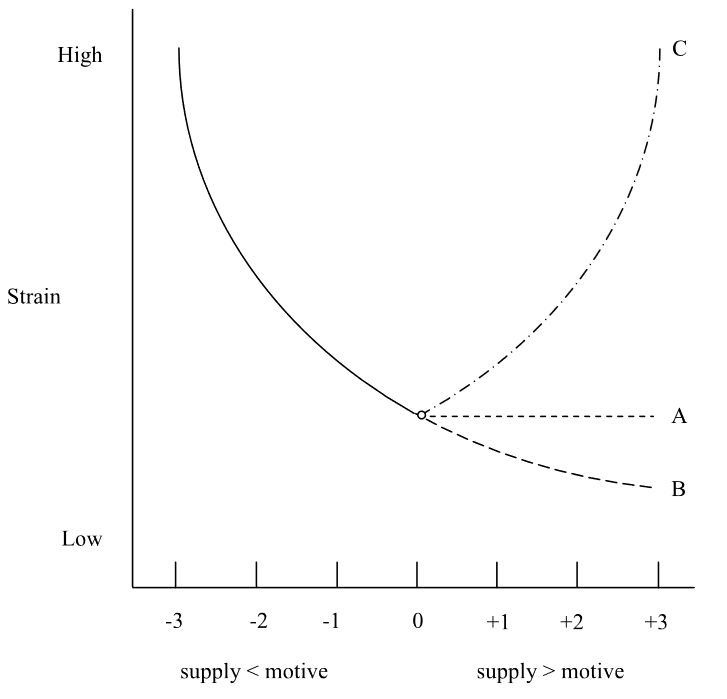
\includegraphics[width=0.75\textwidth]{gfx/ueberschuss_supply_motive.png}
	\caption{Auswirkungen eines Bedürfnisse-Angebote Misfits\\(Eigene Darstellung in Anlehnung an \cite[S. 23]{edwards:2008})}
	\label{fig:methodik:versuchsaufbau:unilateral:abb2}
\end{figure}

Zur Bestimmung des Anforderungen-Fähigkeiten Fits wird angenommen, dass Projektmanager anstreben, offene Projektpositionen mit fachlich optimal passenden Mitarbeitern zu besetzen. Folglich vermeiden sie sowohl eine Über- als auch eine Unterqualifizierung ihrer Angestellten. Aus diesem Grund wird der \ac{PEFit} anhand von Kurve B aus Abbildung \ref{fig:methodik:versuchsaufbau:unilateral:abb2} in der unilateralen Empfehlungskomponente durch quadrierte Differenzberechnung bestimmt.

\newpage
Der Algorithmus der unilateralen Empfehlungskomponente wird anhand der folgenden beispielhaften Projektposition erläutert. (Java: Fortgeschritten, MySQL: Grundkenntnisse; Spark: Grundkenntnisse)

Zu diesem Zweck wird für jede vom Projektmanager geforderte Kompetenz die in Gleichung \ref{fig:personEnvironmentFit:auswirkungenErhoehterAngebote:formel3} vorgestellte quadrierte Differenz zwischen dem Pseudomitarbeiter und allen anderen Angestellten bestimmt. Anschließend werden die Mitarbeiter nach geringster Abweichung sortiert und an den Projektmanager zurückgegeben.

Für die Daten aus Abbildung \ref{fig:methodik:versuchsaufbau:unilateral:abb1} ergibt sich damit die in Tabelle \ref{tbl:methodik:versuchsaufbau:unilateral:tbl2} dargestellte Ausgabe. Die vollständige Berechnung kann in Anhang \ref{ch:nebenrechnungen:unilateral} nachvollzogen werden.

\begin{table}[h]
	\centering
	\begin{tabular}{c|c|c}
		Positionierung & Mitarbeiter & Abweichung\\
		\hline
		1 & Jane D.  & 0.03\\
		2 & Max M.   & 0.08\\
		3 & Erika M. & 0.11\\
		4 & John D.  & 0.16
	\end{tabular}
	\caption{Ergebnisliste der unilateralen Empfehlungskomponente für die Daten aus Abbildung \ref{fig:methodik:versuchsaufbau:unilateral:abb1}}
	\label{tbl:methodik:versuchsaufbau:unilateral:tbl2}
\end{table}

\subsection{Bilaterale Empfehlungskomponente}
\label{ch:methodik:versuchsaufbau:bilateral}

\newpage
Zu erhebende Daten:\\
- Für jeden Mitarbeiter erheben: Wichtigkeit (true/false) --> Auch für Dinge, die man noch nicht kann\\
- Für jeden Mitarbeiter erheben: Welche Auswirkung hat es, wenn im Projekt nicht ausgelastet (Kurve A bis C) --> Alle drei Antwortmöglichkeiten positiv formulieren --> z.B. Freiräume nutzen

Erstellen des Graphen:\\
- Aus Skills (kollaboratives Filtern) und Teamzuordnung (Inhaltsbasiertes Filtern) einen tripartiten Graphen erstellen\\

Eingabe der offenen Projektposition:\\
- Benötigt: Fähigkeiten und Wichtigkeit (Boolean)

Algorithmus:\\
- Berechnung der Katz-Zentralität\\
- Für jeden relevanten Mitarbeiter auf Basis von Abbildung \ref{fig:methodik:abb2} den finalen Wert bestimmen --> Hierbei je nach Wichtigkeit die Kurve stauchen --> Wenn für Projektmanger wichtig, die durchgezogene Linie doppelt so steil; Wenn für Mitarbeiter wichtig, rechte Seite doppelt so steil; Auswahl der Kurve anhand der Information des Mitarbeiters\\
- Summe für alle Fähigkeiten eines Projektes für jeden Mitarbeiter berechnen

\begin{figure}[h]
	\centering
	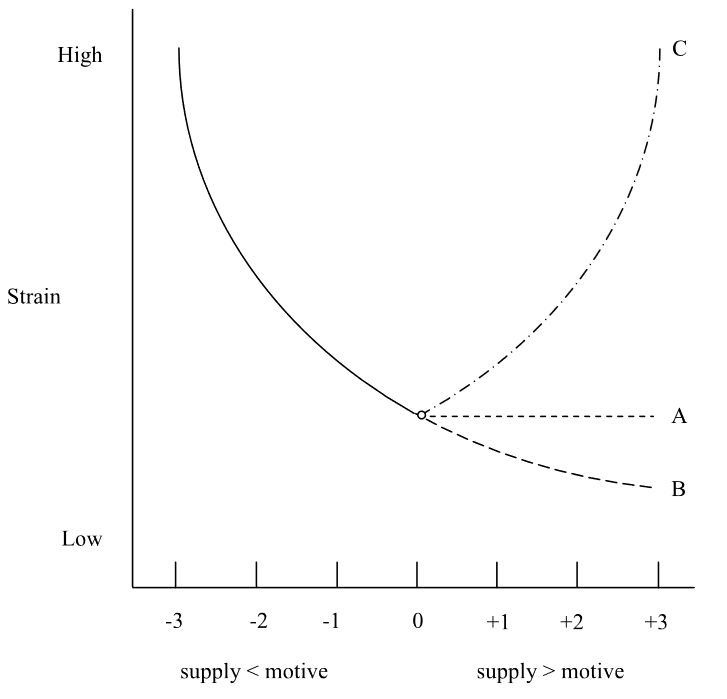
\includegraphics[width=0.75\textwidth]{gfx/ueberschuss_supply_motive.png}
	\caption{Auswirkungen eines Bedürfnisse-Angebote Misfits \cite[S. 23]{edwards:2008}\\(Bearbeitet von \myName)}
	\label{fig:methodik:abb2}
\end{figure}

- Algorithmus einmal durchführen mit Wichtigkeiten und einmal ohne (bilateral vs. unilateral)\\
- Ausgabe der sortierten Liste (mit allen Mitarbeitern (zB 25))\\
- Eingabe der Projektposition und Algorithmus für jede Projektposition wiederholen

\section{Evaluation}
\label{ch:methodik:evaluation}
Evaluation für Projektmanager:\\
- Erhält für jedes Projekt beide Listen und gibt auf einer Skala von 1 bis 5 an, wie hoch der die Leistung der empfohlenen Mitarbeiter in diesem Projekt einschätzen würde

Evaluation für Mitarbeiter:\\
- Jeder Mitarbeiter muss für jedes Projekt auf einer Skala von 1 bis 5 bewerten, wie zufrieden er wäre, wenn er darin arbeiten würde\\
- Ergebnisliste wird in Intervalle geteilt --> z.B. Zufriedenheit 5 bedeutet bei 25 Teilnehmern, dass der Nutzer im ersten Intervall sein muss --> Abweichung bestimmen --> Je weniger Abweichung, desto besser --> Durchschnittliche Abweichung von unilateral und bilateral vergleichen

Es wird bewusst darauf verzichtet, zusätzliche Stellenbeschreibungen oder Auftraggeber zu nennen, die die Bewertung verzerren könnten. Mitarbeiter und Projektmanager erhalten ausschließlich Informationen, die auch vom Empfehlungssystem verarbeitet werden.
\shorthandon{"}